\documentclass[12pt]{article}

\input{../../../../../../_assets/preambulo.tex}
\usepackage{xkeyval} % Para el paso de argumentos

\usepackage{graphicx}

% Definir la carpeta de las imágenes
\graphicspath{{../_assets}{../../_assets}}

% Definir el comando \portada
\makeatletter
\define@key{portada}{titulo}{\def\titulo{#1}}
\define@key{portada}{subtitulo}{\def\subtitulo{#1}}
\define@key{portada}{autor}{\def\autor{#1}}
\define@key{portada}{año}{\def\año{#1}}

\newcommand*{\portada}[1][]{%
    % Definimos las claves y sus valores por defecto
  \setkeys{portada}{%
    titulo=Sin Título,%
    subtitulo=Sin Subtítulo,%
    autor=Autor Desconocido,%
    año=Sin Año, #1}%
    \begin{titlepage}
        \centering
        {\includegraphics[width=0.2\textwidth]{Logo-UGR-Black.png}\par}
        \vspace{1cm}
        {\bfseries\LARGE Universidad de Granada \par}
        \vspace{1cm}
        {\scshape\Large Doble Grado en Ingeniería Informática y Matemáticas \par}
        \vspace{3cm}
        {\scshape\Huge \titulo \par}
        \vspace{3cm}
        {\itshape\Large \subtitulo \par}
        \vfill
        {\Large Autor: \par}
        {\Large \autor \par}
        \vfill
        {\Large \año \par}
    \end{titlepage}%
}

\begin{document}
    \portada[%
    titulo=Fundamentos de Ingeniería del Software,
    subtitulo=Práctica 0,
    autor=Jesús Muñoz Velasco,
    imagen=../../../../../../_assets/Logo-UGR-Black.png,
    año=Curso 2024-2025]

    \tableofcontents

    \newpage

    \section{Diagramas de Casos de Uso}

    \begin{center}
        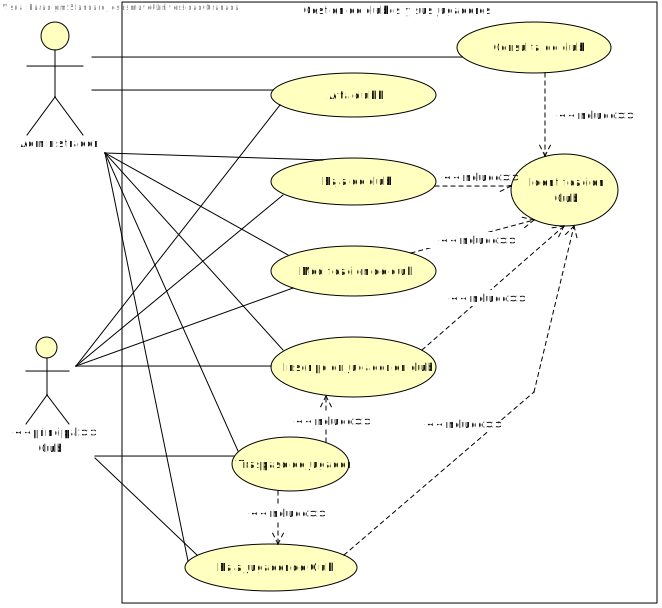
\includegraphics[width=15cm]{../Diagrama de casos de uso.png}
    \end{center}

    \section{Modelo Conceptual}

    \begin{center}
        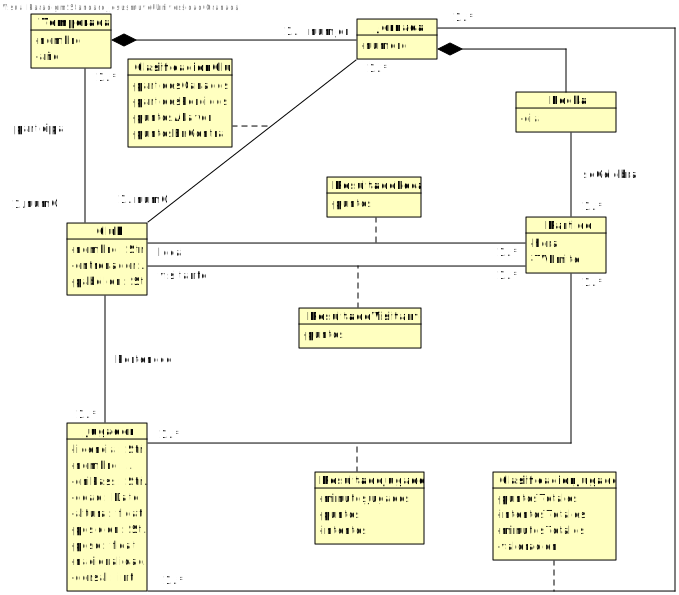
\includegraphics[width=15cm]{../Modelo conceptual.png}
    \end{center}

    \section{Diagrama de Secuencia del Sistema}

    \begin{center}
        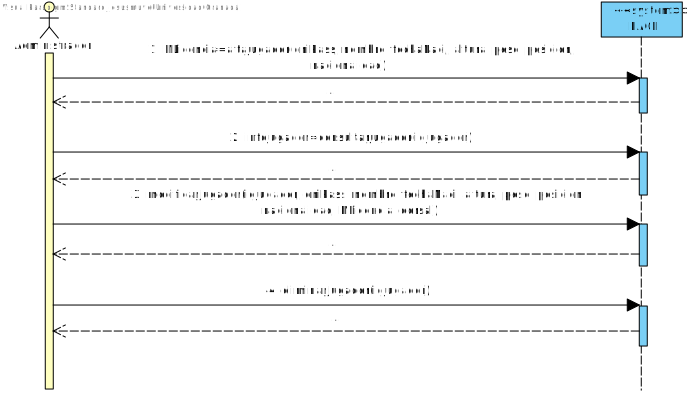
\includegraphics[width=15cm]{../Diagrama de secuencia del sistema.png}
    \end{center}

    \section{Diagrama de Comunicación}

    \begin{center}
        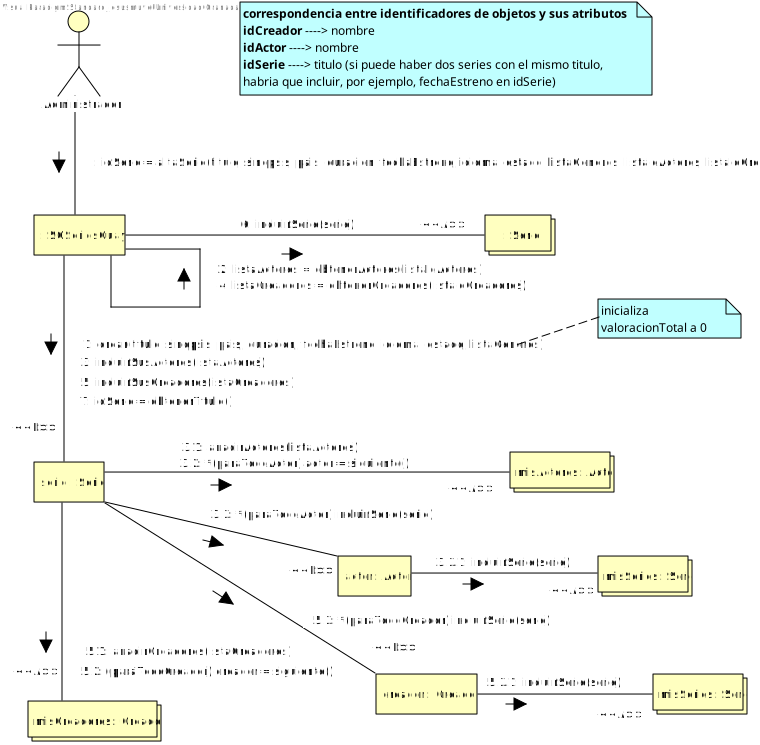
\includegraphics[width=15cm]{../Diagrama de comunicacion.png}
    \end{center}

\end{document}